%************************************************
\section{\LaTeX{}是什么}
\begin{frame}
    \frametitle{\TeX{}}
    \begin{itemize}
        \hidark<1> \item 由Donald E. Knuth (高德纳,唐纳德·克努特) 1977年开始设计
        \hidark<2> \item 由三个希腊字母组成,发音为“Tech”(泰克)
        \hidark<3> \item 最初用于出版工业的数字印刷设备
        \hidark<4> \item 从第3版之后的版本号越来越接近圆周率$\pi$ ,目前的版本是3.1415926
        \hidark<5> \item 非常稳定,高德纳悬赏奖励任何能够在\TeX{}中发现程序漏洞(bug)的人
    \end{itemize}
\end{frame}

\begin{frame}\frametitle{高德纳的传奇}
    \begin{columns}

    	\begin{column}{0.3\textwidth}
        	\begin{figure}[h]
                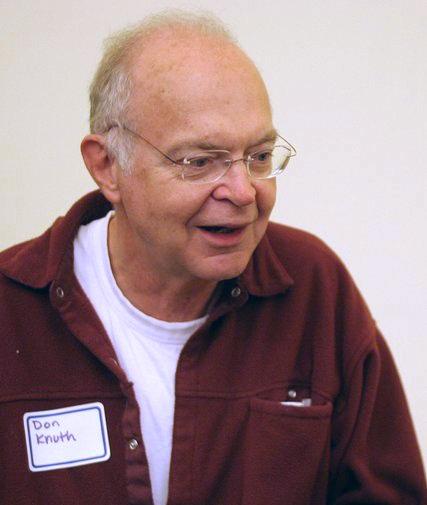
\includegraphics[width=0.9\textwidth]{donald.jpg}
                \caption{高公萌照}
            \end{figure}
    	\end{column}

    	\begin{column}{0.7\textwidth}
        	\begin{itemize}
                \hidark<1> \item 《The Art of Computer Programming》作者
                \hidark<2> \item  美国国家科学院院士
                \hidark<3> \item  美国工程院院士
                \hidark<4> \item  美国艺术与科学院院士
                \hidark<5> \item  斯坦福大学计算机系教授(30岁)
                \hidark<6> \item  最年轻的图灵奖获得者(36岁)
            \end{itemize}
    	\end{column}

    \end{columns}


    \begin{center}
        \footnotesize{\url{http://www-cs-faculty.stanford.edu/~knuth/}}
    \end{center}

\end{frame}

\begin{frame}\frametitle{\LaTeX{}}
    \begin{itemize}
        \hidark<1> \item 发音为“Lay-Tech”(雷态克)
        \hidark<2> \item 由最早由计算机学家Lamport在20世纪80年代初开发
        \hidark<3> \item \LaTeX{} 是在Plain \TeX{}的基础上开发出的一种更为简单的语言
        \hidark<4> \item 提供了预先定义好的专业页面设置
        \hidark<5> \item 短时间内生成具有书籍质量的印刷品
        \hidark<6> \item 还可以用来生成矢量图形
    \end{itemize}
\end{frame}

\begin{frame}\frametitle{\LaTeX{}优点}
    \begin{itemize}
        \item<1-> \textcolor{red}{模板漂亮}。让你的文档足够漂亮以应对各种场合-
        \item<2-> \textcolor{red}{编写方便}。可以容易地编辑公式、生成脚注、索引、目录、参考文献等复杂的文档结构
        \item<3-> \textcolor{red}{省时省力}。可以免去很多费力不讨好的页面样式设计工作
        \item<4-> \textcolor{red}{资源丰富}。有大量的模版可以借鉴,很容易套用
        \item<5-> \textcolor{red}{统一标准}。\LaTeX{}是科研界标准,很多期刊提供模板,甚至提供在线编译功能
        \item<6-> \textcolor{red}{当前国情}。用\LaTeX{}写算法导论报告分数会高一些
        \item<7-> \textcolor{red}{业界良心}。体会码农的乐趣
    \end{itemize}
\end{frame}

\begin{frame}\frametitle{\LaTeX{}缺点}
    \begin{itemize}
        \hidark<1> \item 不是所见即所得,上手不如word简单,但是一劳永逸。
        %有人把时间花在了重复工作上,有人花了积累模板上。一两年以后,前者依旧,后者不再需要花时间。
        \hidark<2> \item 组织结构混乱的文章不太容易写,但我们追求的就是清晰的结构。
        \hidark<3> \item 自己重新设计整个排版很花时间,但我们没有设计排版的需求。
        \hidark<4> \item 很难做出很花哨的效果,但我们不会去做花哨的效果。
    \end{itemize}
\end{frame}

\begin{frame}\frametitle{\LaTeX{} vs Word}{——能抓到老鼠的猫就是好猫}
    \begin{figure}[h]
        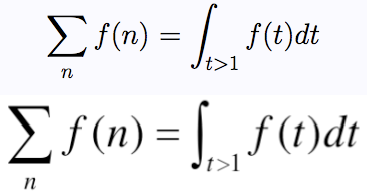
\includegraphics[width=0.4\textwidth]{latex_word.png}
    \end{figure}
    \begin{itemize}
        \hidark<2> \item \LaTeX{}各种字母体型优美,仪态万方
        \hidark<3> \item 文档大小较之Word小很多,并且是文本格式
    \end{itemize}
\end{frame}

\begin{frame}\frametitle{接下来要介绍的内容}
    \begin{itemize}
        \hidark<1> \item helloworld.tex
        \hidark<2> \item 基本语法介绍
        \hidark<3> \item 章节、段落
        \hidark<4> \item 数学公式
        \hidark<5> \item 插入代码、图片、表格和引用
        \hidark<6> \item 中文支持
        \hidark<7> \item Beamer(Slides NOT PPT)
        \hidark<8> \item 参考文献的加入
        \hidark<9> \item 几个省事的软件
    \end{itemize}
\end{frame}